\documentclass{article}

\usepackage[utf8]{inputenc}
\usepackage[english]{babel}
\usepackage{float}
\usepackage{fancyhdr}
\usepackage{amsmath}
\usepackage{color}
\usepackage{listings}
\usepackage{graphicx}
\usepackage{pdfpages}
\usepackage{booktabs}
\usepackage{listingsutf8}
\usepackage[a4paper, top = 1in, bottom = 1in, left=1.5in,right=1.5in]{geometry}
\usepackage[backend=biber, citestyle=ieee]{biblatex}
\usepackage{csquotes}
\usepackage{hyperref}
\usepackage{enumitem}

\bibliography{ai.bib}

\title{Notes for AI}
\author{Peter Heilbo Ratgen}
\date{\today}

\hfuzz=80pt


\begin{document}
\maketitle

\tableofcontents

\newpage

\section{Week 5 February - Introduction}%
\subsection{Basics}
The course is an introduction to the basics of Artificial Intelligence. We will
get an overview of the base of the artificial intelligence methods. We will use
python as a programming language. Labs and support will be done in python.
Prerequisite to the exam is to complete the homework of the lectures.
\cite{book:artificial_intelligence_modern_approach}

You should help each other, but coding should be done individually.
\begin{itemize}
  \item Thinking humanly
  \item Acting humanly
  \subitem The Turing test is used to test this. The longer a human can be
  fooled into thing that the human is talking to a human, and not a bot.  This
  could be chatbots acting humanly. You have to test for:
  \begin{itemize}
    \item Natural language processing
    \item Knowledge representation
    \item Automaed reasoning\
    \item Machine learning
  \end{itemize}
    Success depends on deception. Chatbot can use cheap tricks. Mitzuku has
    recently won for the 5th time.
    Computers have a had time with multiple choice questions. Eg the "The large
    ball crashed right through the table because it was made of styrofoam". If
    you replace "styrofoam" with "steel", then the answer is totally different.
    
    \textbf{A better test?} A better Turing test, would be one that can be
    administed and graded by a machine, and more objectivity in the it would not
    depend of subjectity of humans.

  \item Thinking rationally
    \subitem
    It is about the idealized or "right" way of thinking. It is hard to describe
    the world using logical notation. The procedure of applying these local
    statements and deducing them. 
    We also have a though time dealing with uncertainty, representing the gray
    areas.
  \item Acting rationally
    \subitem
    Acting rationally is acting with the goal of achieving the goal, that has
    been set. Utility is about the goal that has been set, whether it is about,
    shortest route, least time or fewest changes in a public transit system.
\end{itemize}
\subsection{Successes of AI}
\begin{itemize}
  \item IBM Watson is an AI created by IBM. IBM is one of the companies that has been
investing in AI for the longest times. 
  \item Self driving cars is one of the successes of AI. This is an example of a
  rational acting. 
  \item Natural language processing is also a great improvement, with speech
technologies and machine translation.
  \item Vision, OCR, handwriting recognition and face detection and recognition.
  \item Mathematics, program solved unsolved conjecture. Also wolfram alpha.
  \item Games
    \subitem Chess(champion beaten in 1997), checkers(solved in 2007), Go
    (beaten for the first time by a Google AI), Google AI beat top StarCraft
    players.
  \item Logistics, scheduling, planning.
    \subitem A lot of the advancement are done by the military. In the 1991 Gulf
    War an AI planned and scheduled for 50,000 vehicles and such.
  \item Robotics
    \subitem Mars rovers, self driving cars, drones, robot soccer, personal
    robotics.
\end{itemize}



Exercises will start at 10:20.
\paragraph{Basics}
Python code is fairly simple and readable. Beginning and ending of blocks is
done purely by indentation. We will use the Python Console for trying out
examples. Variables can change types throughout the program. A variable can
start as a string end as float. We can use \texttt{+} for string concatenation.
We can use triples quotes for strings containing both \texttt{'} and \texttt{"}.

Variables in Python do not have intrinsic types. But assignment does not create
copies, but references. References are deleted by the garbage collector, when
the reference has passed out of scope. Names cannot start with numbers.

We can have multiple assignments. And swapping vars is easy.
\begin{lstlisting}
>>> x, y = 2, 3
>>> y
3
>>> x, y = y, x
>>> y
2
>>> x
3
\end{lstlisting}

\subparagraph{Sequence types}
Sequence types are tuples, strings and lists. In a tuple we can have multiple
types of variables. Tuples are immutable, such that they cannot be changed after
it has been created. Strings are also immutable. Lists are mutable, they can
also have mixed types.
These sequence types have much syntax in common. If we have to change elements
in an immutable tuple or string a new copy has to be created. Lists can be
shrunk or expanded as you go. We assign some different variables:

\begin{lstlisting}[inputencoding=utf8/latin1,basicstyle=\ttfamily,
language=python, keywordstyle=\color{blue}\bfseries, rulecolor=\color{black}]
>>> tu = (23, 'abc', 4.56, (2,3), 'def')
>>> tu
(23, 'abc', 4.56, (2, 3), 'def')
>>> li = ['abc', 34, 4.34, 23]
>>> st = "Hello World"
>>> st
'Hello World'
>>> st = Helllo wordl'
  File "<stdin>", line 1
    st = Helllo wordl'
                ^
SyntaxError: invalid syntax
>>> st = 'Helllo wordl'
>>> st
'Helllo wordl'
>>> st = """THis is a multiple line
... string that uses triple quotes"""
>>> st
'THis is a multiple line\nstring that uses triple quotes'
\end{lstlisting}
We can also have negative indexes, such that -1 is the last character:
\begin{lstlisting}[inputencoding=utf8/latin1,basicstyle=\ttfamily,
language=python, keywordstyle=\color{blue}\bfseries, rulecolor=\color{black}]
>>> st[-1]
's'
>>> st[-2]
'e'
\end{lstlisting}
If want to get the 3 middle elements of the tuple we defined:
\begin{lstlisting}[inputencoding=utf8/latin1,basicstyle=\ttfamily,
language=python, keywordstyle=\color{blue}\bfseries, rulecolor=\color{black}]
>>> tu[1:4]
('abc', 4.56, (2, 3))
\end{lstlisting}
From this we get a \underline{copy} of the selected part of the tuple. If we do
not specify where in the tuple to start, we start from the beginning.
\begin{lstlisting}[inputencoding=utf8/latin1,basicstyle=\ttfamily,
language=python, keywordstyle=\color{blue}\bfseries, rulecolor=\color{black}]
>>> tu[:3]
(23, 'abc', 4.56)
\end{lstlisting}
We can do a copy like this:
\begin{lstlisting}[inputencoding=utf8/latin1,basicstyle=\ttfamily,
language=python, keywordstyle=\color{blue}\bfseries, rulecolor=\color{black}]
>>> tu[:]
(23, 'abc', 4.56, (2, 3), 'def')
\end{lstlisting}

In this example there is a big difference between line 3 and 4.
\begin{lstlisting}[inputencoding=utf8/latin1,basicstyle=\ttfamily,
language=python, keywordstyle=\color{blue}\bfseries, rulecolor=\color{black}]
>>> l3 = ['4', '5']
>>> l4 = ['6', '7']
>>> l3 = l4
>>> l3 = l4[:]
\end{lstlisting}
In line 3 we assign \texttt{l3} we assign to the reference to \texttt{l4}. In
the 4th line we assign \texttt{l3} to a \underline{copy} of \texttt{l4}, such
that changes in \texttt{l4} will not be reflected in \texttt{l3}.

We can use the \texttt{in} operator to check if we have a substring. We can
concat tuples:
\begin{lstlisting}[inputencoding=utf8/latin1,basicstyle=\ttfamily,
language=python, keywordstyle=\color{blue}\bfseries, rulecolor=\color{black}]
>>> tu[:] + tu2[:]
(23, 'abc', 4.56, (2, 3), 'def', 12, 'yeet')
>>> tu + tu2
(23, 'abc', 4.56, (2, 3), 'def', 12, 'yeet')
\end{lstlisting}

\subparagraph{Dictionaries}
Dictionaries can store a mapping between a set of keys and values. We can
create a dictionary with:
\begin{lstlisting}[inputencoding=utf8/latin1,basicstyle=\ttfamily,
language=python, keywordstyle=\color{blue}\bfseries, rulecolor=\color{black}]
>>> d = {'user' : 'bozo', 'pswd' : 1234}
\end{lstlisting}
The values can be anything. We can get the value of a key like this:
\begin{lstlisting}[inputencoding=utf8/latin1,basicstyle=\ttfamily,
language=python, keywordstyle=\color{blue}\bfseries, rulecolor=\color{black}]
>>> d['user']
'bozo'
\end{lstlisting}
We can delete a key:value pair like this:
\begin{lstlisting}[inputencoding=utf8/latin1,basicstyle=\ttfamily,
language=python, keywordstyle=\color{blue}\bfseries, rulecolor=\color{black}]
>>> del d['pswd']
>>> d
{'user': 'bozo'}
\end{lstlisting}

\newpage

\section{Week 7 - Intelligent Agents}
An agent is anything that can be viewed as perceiving its environment through
sensors and acting upon that environment through actuators. We can say that
an agents behaviour is described by its \textbf{agent function}. This maps any sequence
to an action. This is a mathematical abstraction, the \textit{actual program} is
called the \textbf{agent program}. \cite[p. 3]{presentation:intelligent_agents}

We can have many types of agents, these can perceive in many ways: here are some
examples.
\begin{itemize}
  \item Human agent
    \subitem Eyes, ears, nose
  \item Robotic agent
    \subitem Cameras, and infrared range finders
  \item Software agent
    \subitem Keystrokes, file contents \& network packets.
\end{itemize}

\subsection{Vaccum-cleaner world}%
\label{sub:vaccum_cleaner_world}
A vecuum-cleaner has two locations to take care of: A and B. It has four
actions: left, right, such and NoOp. We can have a simple programme for cleaning
with this vaccum:

\begin{lstlisting}
if status = Dirty then return Suck
else if Location = A then return Right
else if Location = B then return Left
\end{lstlisting}

The vacuum-cleaner is a rational agent, it tries to optimize on a performance
measure. The choice of performance measure is a critical one. "Doing the right
thing" is to always act according to the performance measure. We also call the
performace measure the utility function, it is an objetive criteria for the
success of an agent's behaviour.

An example of potential performance measures for the vacuum agent.
\begin{itemize}
  \item amount of dirt cleaned up
  \item amount of time taken,
  \item amount of electricity consumed
  \item amount of noise generated
\end{itemize}
It would be desirable to have the agent take as little time as possible, but if
we only consider this, then it would stand still. But if combined, with eg the
amount of dirt cleaned up, then we could have beter operation.

\subsection{Autonomy}%
\label{sub:autonomy}
An autonomous agnet always has the ability to learn and adapt, it can always say
"no", it also needs enough built-in knowledge to survive.

\paragraph{Task Environment Specification}
Problem specification:
\begin{itemize}
  \item Performace meassure
  \item Environment
  \item Actuators
  \item Sensors
\end{itemize}
For a autonomous taxi
\begin{itemize}
  \item Performace meassure
    \subitem Safe, fastm, legal
  \item Environment
    \subitem Roads
  \item Actuators
    \subitem Steering wheel
  \item Sensors
    \subitem Cameras, speedometer
\end{itemize}

For an email spam filter:
\begin{itemize}
  \item Performace meassure
    \subitem Manimizing false positives
  \item Environment
    \subitem User email account
  \item Actuators
    \subitem Mark as spam, let mail through
  \item Sensors
    \subitem Incoming messages
\end{itemize}

\subsection{Environment types}%
\label{sub:environment_types}
\paragraph{Fully observable vs partially observable}
In a games, such as FIFA or any game, it is possible to oberserve everything,
and perceive all options.
If a robot is playing football in the real world, then the perception of the
environment is constrained by the input of the sensors eg eyes (you do not know
what happens behind your back).

\paragraph{Deterministic vs stochastic}
A deterministic environment is when the coming events in time is only defined
by the current state, and the agent's future actions. Versus when the game is
dependent on some type of randomness, whether it be a deck of cards or dice.
This is very hard to predict.

\paragraph{Episodic vs sequential}
Is every step of the agent independent? Or does it depend on a previous
sequence? A sequence could be a game, where current decisions depend on a 
previous sequence of decisions. In a spam filter the sequence of spam mail does
not matter.
This is a matter of defintion, it is how you see your environment in terms of
your decisions. A game could be episodic, if you choose to look upon it as a
snapshot.

\paragraph{Static vs dynamic}
Is the world changing while the agent is thinking. Solving a rubrics cube or
chess is static. However self-driving is very dynamic, here things are changing
all the time. This a very challenging 


\paragraph{Discrete vs continuous}
Does the environment provid a fixed number of distinct number of states(can they
be enumerated)? Where time is a factor, then time is always continuous, if you
do not choose to look at time in buckets of seconds or minutes.

\paragraph{Single-agent vs multiagent}%
\label{par:single_agent_vs_multiagent}
Is the agent operating by itself?

\subsection{Hierarchy of agent types}%
\label{sub:hieryachy_of_agent_types}
\begin{itemize}
  \item Table-driven agents, it's just like a big lookup table. 
    \subitem The table sizes can become huge. Designing such a table is
    challenging. We need to think about every single case.
  \item Simple reflex agent
    \subitem This is the vacuum cleaner. For every state given the rules, we
    find the rule applying to the current state. It selects its action from the
    current percept only. Implemented through condition-action rules. Example of
    if-then algorithms. For this to work, then the environment must be fully
    observable. This wont then work for a self-driving car.
  \item Agents with memory, internal state to keep track of past states of the
    world
    \subitem We can call this a model-based reflex agent. Internal state:
    aspects of the environment that cannot be currently observed. This is useful
    for partially observable environments.
    In addition to the rule we have a model, a desripton of how the next state
    depends on current state and action.
    We also have a state, a description of the current world state
    the action, is the most recent action.

    We update the state, according to the state, action, percept and the model.
    When matching a rule, the we take into account the state and the rules.
  \item Agents with goals
    \subitem 
  \item Utility 
\end{itemize}


\newpage


\section{Week 8 - Uninformed Search}

\subsection{Formulating search problems}%
\label{sub:formulating_search_problems}

Many problems can be solved through search. Which sequence of actions can get us
to the goal state? This can be solved through search. We might also have a
performance measure of minimizing time. For an example a GPS is a search
problem, which sequence of places gets us to the goal?
\cite[p. 2]{presentation:solving_problems_by_searching}

There can be many different examples of using search as a solution to a problem.
Examples are getting somewhere, we can formulate the problem as:
\begin{itemize}
  \item Start: home
  \item Goal: destination
  \item operators: move one block, turn
\end{itemize}


We can also formulate getting settled in a new apartment as a search problem.
\begin{itemize}
  \item start: item randomly distributed over the place
  \item goal: satisfactory arrangement of items
  \item operators: select item, move item
\end{itemize}

\subsubsection{Searching}%
\label{ssub:search}

A search algorithm will tell us the exact sequence to get us from the start to
the goal. Search strategies are important methods for many approaches to
problem-solving. Search algorithms is a basis for many optimization and planning
methods.

We will consider the problem of designing goal based agent in observable (the
agent always knows the current state), deterministic (that each action we take
has exactly one outcome), discrete (that we have finite number of actions to
choose from), known (such that the agent knows which states are reached by each
action) environments\cite[p. 66]{book:artificial_intelligence_modern_approach}. 


\paragraph{State Space}
Is the initial state, actions and the successor function (or transition model)
defines the state space of the problem.  The set of all states reachable from
initial state by any sequence of actions.  This can be represented as a directed
graph (nodes are states and the edge between nodes are actions).  

\paragraph{Building a goal based agent}

To build a goal based agent, we must answer the questions\cite[p.
15]{presentation:solving_problems_by_searching}:
\begin{itemize}
  \item How to we represent the state of the world?
  \item What is the goal and how can we recognize it?
  \item What \textit{relevant} information do we encode to describe states,
    action and therir effects aand thereby solve the problem.
\end{itemize}

\subsection{Examples of search problems}

How we solve a comic-book maze.
\begin{itemize}[noitemsep]
  \item solution fixed sequence of actions 
  \item Search: process  of looking for the sequence of of actions that reaches
    the goal
  \item Agent can ignore percepts during execution.
\end{itemize}

\paragraph{The maze problem}

To solve a maze by searching we examine the components of a search problem.
\cite[p. 8]{presentation:solving_problems_by_searching}

\begin{itemize}[noitemsep]
  \item Initial state 
    \subitem Entry 
  \item Successor Function
    \subitem Is the result of the doing an action in a state
  \item Goal state 
    \subitem Goal state is the exit.
  \item Path cost
    \subitem Assume that it is a sum of nonnegative \textit{step costs}.
  \item Optimal solution: sequence of actions with the lowest path cost.
\end{itemize}

The optimal solution is the sequence of actions with the \textit{lowest path
cost} for reaching the goal.

\paragraph{Vacation in Romania} 
We are on vacation in Romania, currently we are placed in Arad. However our flight
leaves Bucharest tomorrow. Now we want to find the best way to get to Bucharest.

\begin{itemize}[noitemsep]
  \item Initial state
    \subitem Arad
  \item Successor function 
    \subitem These are the possible states we can move to $S(\text{Arad}) = \{\text{Zerind}, \text{Timisoara}, \text{Sibiu}\}$
  \item Goal state
    \subitem Bucharest
  \item Path cost
    \subitem The cost of the path from the start to the goal, is the sum of edge
    costs.
\end{itemize}

We find the graph on \cite[p. 9]{presentation:solving_problems_by_searching}.

\paragraph{Vaccum-cleaner world}
We can define a state for the vaccum world:
\begin{itemize}[noitemsep]
  \item Initial state 
    \subitem Dirty
  \item Goal state
    \subitem All clean
  \item State space:
    \subitem 
    \begin{figure}[H]
      \center
      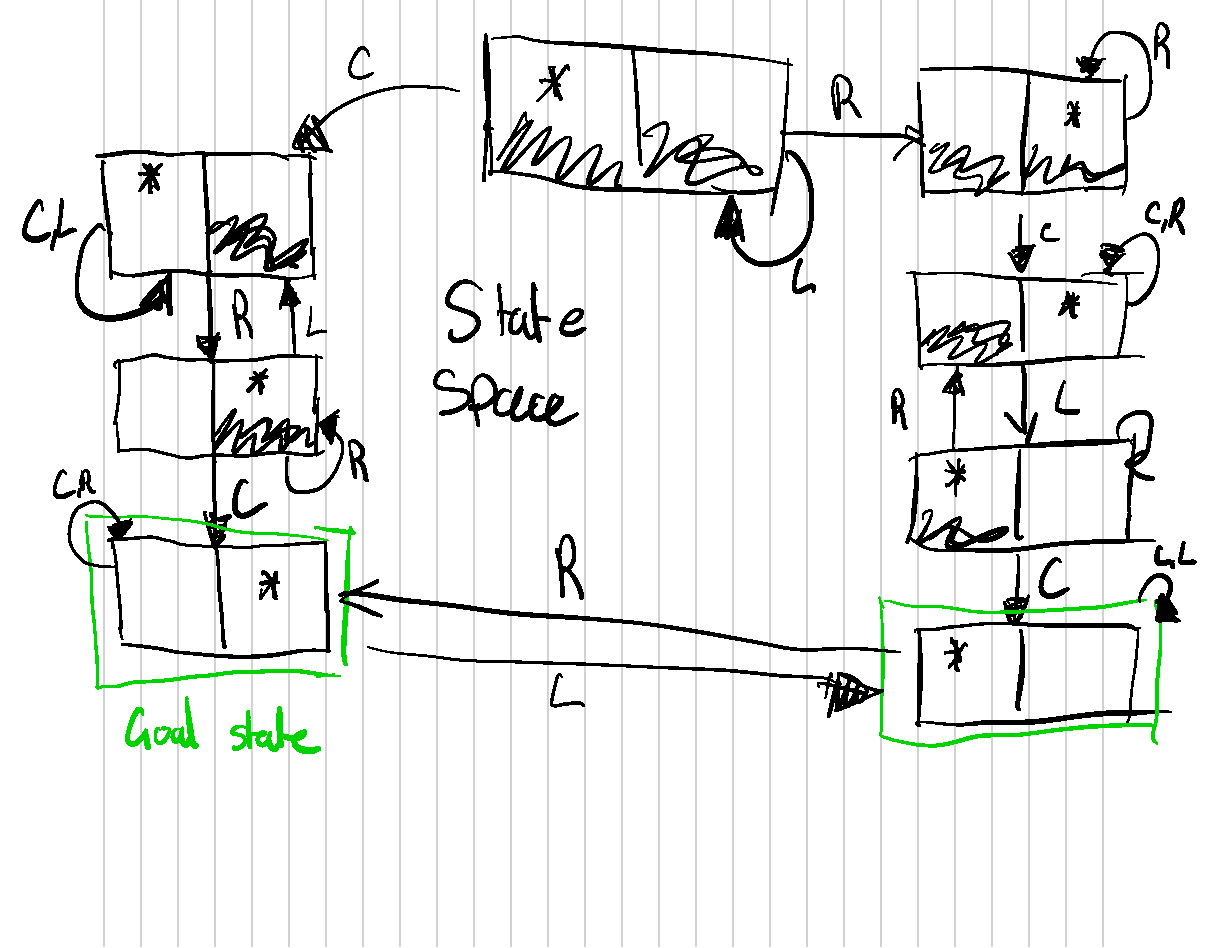
\includegraphics[width=0.7\textwidth]{./statespace.pdf}
      \caption{The state space of the vacuum cleaner world}
    \end{figure}
  \item Path cost
    \subitem Could be the sum of the amount of electricity used, or any other
    type of utility function.
\end{itemize}

\paragraph{Example: The 8-puzzle}
The state space of the 8-puzzle has a size of 181440 states. The successor
function is the actions of move blank left, right, up, down. The optimal
solution is NP-hard\cite[p. 17]{presentation:solving_problems_by_searching}.

\paragraph{Example: The 8-queens problem}
On chessboard 8 queens are placed. We must place the queens, such that no other
queen can attack each other. 
\begin{itemize}
  \item State space: Is the chessboard
  \item Successor function: depends on how you want to formalize it. It could be
    moving one piece in a direction, such that you have a different
    configuration.
  \item Goal state: Check if any queen is on the same row, column or diagonal.
\end{itemize}

\paragraph{Example: Remove 5 sticks}
Remove exactly 5 of the 17 stick such that the result forms 3
squares \cite[p. 18]{presentation:solving_problems_by_searching}.

\begin{itemize}
  \item States: 
  \item Initial state: The initial state is the state presented with all the
    sticks laid out, and having the 6 squares.
  \item Successor function: Picking up any stick from the board.
  \item Goal test: Check if the remaining sticks form the 3 squares, we need to
    have a function for that.
  \item Path cost: It cost one to remove a stick.
\end{itemize}


\subsection{Tree search}

We expand at the root node(which is the starting state). As we go about
expanding the tree of the search, we maintain a list of unexpanded nodes. This
we call the fringe. For each iteration we expand a node we pick from the fringe.
We keep expanding until we reach the goal state. Our \textbf{goal} is to expand
as few states as possible. This is the case as it takes time and can fill up the
memory of the computer.

An important point is to that \emph{nodes and states} are not the same. A state
is a representation of a physical configuration, while a node is a data
structure that is par of the search tree\cite[p.
19]{presentation:solving_problems_by_searching}

A tree search algorithm works in the following way:
\begin{enumerate}
  \item Initialize the fringe with the starting state
  \item As long a the fringe is not empty:
    \begin{enumerate}
      \item Choose a fringe node to expand
      \item If the node contains the goal state, then return that solution
      \item If not, expand the node and add the children of this node to the
        fringe.
    \end{enumerate}
  \item If we reach the end, terminate having found no solution.
\end{enumerate}
We keep an explored set of the node we already have visited, a node is added to
this everytime we expand it. When we add a node to the fringe, then we check if
it exists, with a higher path cost. If this is the case, then replace it.

\subsection{Search strategies}%
\label{ssub:search_strategies}

A search strategy is defined by the order in which we pick which node to expand
from the fringe. We have some different parameters by, which to judge a search
strategy:
\begin{itemize}[noitemsep]
  \item Completeness
    \subitem Does it find a solution if it exists?
  \item Optimality
    \subitem Does it find the cheapest solution?
  \item Time complexity
    \subitem This represents the number of the node generated aka the time it
    take to run.
  \item Space complexity
    \subitem How many nodes are in memory?
\end{itemize}
We can measure the time and space complexity in terms of:
\begin{itemize}
  \item $b$: maximum branching factor of the search tree
  \item $d$: depth of the least cost (cheapest) solution.
  \item $m$: maximum length of any path in the state space (could be unbounded).
\end{itemize}

\subsubsection{Breadth-first search}%
\label{par:breadth_first_search}
We expand the shallowest node, such that we search in the breath of the tree.
This is done by the fringe being made as a first in-first out queue. Such each
node that we expand, goes to the end of the fringe list.

\begin{description}
  \item[Compleness] Yes
  \item[Optimality] Yes - if the cost is 1 for each step.
  \item[Time complexity] Number of node in a $b$-ary tree of depth $d$: the
    complexity is $O(b^d)$. Where $d$ is the depth of the optimal solution.
  \item[Space complexity] $O(b^d)$
\end{description}

\subsubsection{Depth-first search}%
\label{par:depth_first_search}
We expand the deepest node first, such that we traverse the depth of the tree,
before visiting node higher up. This is done as a last-in-first-out queue.

\begin{description}
  \item[Compleness] Cannot deal with infinte depths, and space with loops. We be
    complete in finite space, if repeats are excluded from the list of visited
    nodes.
  \item[Optimality] No - it returns the first solution that it finds.
  \item[Time complexity] At depth $m$: $O(b^m)$.
  \item[Space complexity] $O(bm)$
\end{description}

\subsubsection{Iterative deepening search}%
\label{par:iterative_deepening_search}
This is a mix of depth first, and breadth-first. We first examine the tree in a
depth-first with the depth of 1 (we cut off node on level 2 and below). If we do
not find out solution we run again with a depth of 2. We again search in a depth
first-fashion. It is like having a depth-first approach, but find an optimal
solution. This way we cannot fall into infinte loops.


\subsubsection{Uniform-cost search}%
\label{par:uniform_cost_search}
We organise the fringe such that all node are sorted according to the cost. Such
that when we expand the root node, then its children B (cost 5) and D (cost 3)
are sorted in the order D, B. We then go on to expand D.

Note that \cite[p. 33]{presentation:solving_problems_by_searching} says that we
should keep expanding nodes in the fringe until we are about to expand the goal
node, and we should \textbf{not} stop when encountering it. Because there might
a hidden better solution in the last unexpanded nodes.



\newpage



\section{Week 9 - Informed Search}%
\label{sec:1_march_informed_search}

\newpage
\section{Week 10 - Local Search}
We can formulate problems in terms of optimization. We do not care about the
path to a solution. We have an objective function that us about the quailt of a
possible solution, and we want to find a good solution by minimizing or
maximizing the value of the function.

There is three approaches to local search.

\subsection{Hill-climbing (greedy) search}
Here the crux is: keep a single "current state" and try to locally improve it.
You can like it to "climbing mount Everest in thick fog with amnesia".

If we look at a puzzle, it should be 1, 2, 3, 4, 5, 6, 7, 8 going in a clockwise
circle our function is $$f(n) = -(\text{number of tiles out of place})$$.
We want to find the best solution, the one closest to what we think we want.

In each iteration we probe, for which move increases our evaluation function.
It can get stuck in a local optimum.

\subsection{Simulated annealing search}
The hill-climbing will be never go down the hill of global and local maxima. 
The idea is to escape local maxiam by allowing some "bad" moved but gradually
decrease the frequency of these bad moves.
\begin{itemize}
  \item Probability of takeing downhill move decreases with number of
    iterations, steepness of downhill move
  \item Controlled by annealing schedule 
\end{itemize}
Inspired by annealing process, as part of the tempering of glass, metal.



\newpage
\section{Week 11 - Adversarial Search}%
\label{sub:_adversarial_search}


\newpage
\section{Week 12 - Constraint Satisfaction Problems}%
\label{sec:23_march_constraint_satisfaction_problems}



\newpage
\section{Week 15 - Probability}%
\label{sec:12_march_probability}

\newpage
\section{Week 16 - Bayesian Networks}%
\label{sec:20_march_bayesian_networks}

\newpage
\section{Week 17 - Hidden Markov Models}%
\label{sec:27_march_hidden_markov_models}

\newpage
\section{Week 18 - Intro to Machine Learning}%
\label{sec:}

\newpage
\section{Lab 1 - Week 7}%
\label{sec:lab_week_7}

\subsection{TABEL-DRIVEN-AGENT}%
\label{sub:tabel_driven_agent}

\paragraph{Run the module}
The program prints:

\paragraph{The percept }

\newpage
\section{Lab 2 - Week 8}%
\label{sec:lab_week_8}

\begin{enumerate}
  \item Successor nodes are inserted at front of the fringe (successor list) as
    a node is expanded. Is this a breadth (FIFO) or depth-first search (LIFO)?
    \subitem This is depth-first search. We put the successor node in front, and
    examine these first.

  \item For goal J, give the fringe (successor list) after expanding each node.
    \subitem The fringe list, should be empty, when we have found the goal J.
    However if we just expand the tree, going depth-first with LIFO then we
    would have: 
    \begin{center}
      J I H G F C E D B A 
    \end{center}
  \item What is the effect of inserting successor nodes at the end of the fringe
    as a node is expanded? A depth or breadth-first search?
    \subitem The effect of this is a breadth-first search.
  \item For goal J, give the fringe (successor list) after expanding each node
    \subitem A, B, C, D, E, F , G, H, I, J
\end{enumerate}

\newpage
\section{Lab 3 - Week 9}%
\label{sec:lab_week_9}


\newpage
\section{Lab 4 - Week 10}



\newpage
\section{Lab 5 - Week 11}


\newpage
\section{Lab 6 - Week 12}

\newpage
\printbibliography

\end{document}

